\documentclass[11pt,a4paper]{article}
\usepackage{algorithm, algorithmic, listings} % Code
\usepackage{amsmath,mathtools,amssymb,amsfonts,dsfont,cancel} % Math
\usepackage{amstext}
\usepackage{color, xcolor} % Color
\usepackage{diagbox, tabularx} % Table
\usepackage{enumerate} % List
\usepackage{epsfig, epstopdf, graphicx, multicol, multirow, palatino, pgfplots, subcaption, tikz} % Image.
\usepackage{fancybox}
\usepackage{verbatim}

\usepackage[font=footnotesize]{caption} % labelfont = bf
\usepackage[font=scriptsize]{subcaption} % labelfont = bf
\usepackage[margin=1in]{geometry}
\usepackage[hidelinks]{hyperref}
\epstopdfsetup{outdir=./Figure/Converted/}
\graphicspath{{./Figure/}{./Figure/part_ii_q_3}{./Figure/part_ii_q_4}{./Figure/part_iii_q_3}}

\makeatletter
\def\input@path{{./Figure/}}
\makeatother

\pgfplotsset{compat=1.13} 

% MATLAB
\lstset{extendedchars=false, basicstyle=\normalsize\tt, language=Matlab, tabsize=4, numbers=left, numberstyle=\small, stepnumber=1, numbersep=8pt, keywordstyle=\color[rgb]{0,0,1}, commentstyle=\color[rgb]{0.133,0.545,0.133}, stringstyle=\color[rgb]{0.627,0.126,0.941}, backgroundcolor=\color{white}, showspaces=false, showstringspaces=false, showtabs=false, frame=single, captionpos=t, breaklines=true, breakatwhitespace=false, morekeywords={break, case, catch, continue, elseif, else, end, for, function, global, if, otherwise, persistent, return, switch, try, while}, title=\lstname,
mathescape=true,escapechar=? % escape to latex with ?..?  
escapeinside={\%*}{*)}, % if you want to add a comment within your code  
%morestring=[m]', % strings
%columns=fixed, % nice spacing
}

\begin{document}
\title{\sc\vspace{3cm}\hrule\vspace{0.3cm}{\LARGE EL2320}\\\vspace{0.1cm}{\Large Applied Estimation}\vspace{0.3cm}\hrule\vspace{1.5cm}{\Large Laboratory Report}\\{\large Lab 1: Extended Kalman Filter}}
\author{{\small Jiang, Sifan}\\{\small sifanj@kth.se}}
\maketitle
\newpage

\newcounter{cnt_questions}
\setcounter{cnt_questions}{0}
\section{Preparatory Questions}
\par \textbf{Linear Kalman Filter:}
\begin{enumerate}
\setcounter{enumi}{\arabic{cnt_questions}}
	\item \addtocounter{cnt_questions}{1} What is the difference between a 'control' $\mathbf{u_{t}}$, a 'measurement' $\mathbf{z_{t}}$ and the state $\mathbf{x_{t}}$?  Give examples of each?
		\begin{itemize}
			\item $\mathbf{u_{t}}$ contains information about the change of the state in the environment. Control is part of dynamic model between $\mathbf{x_{t-1}}$ and $\mathbf{x_{t}}$. For example: velocity of a robot.
			\item $\mathbf{z_{t}}$ measures data through sensor measurements. The data is about the state of its environment. Measurement is modeled as depending on the state at time $t$ with function $\mathbf{h(x_{t})}$. For example, range scans.
			\item $\mathbf{x_{t}}$ is used to describe environments which in the case of robot is the collection of all aspects of the robot and its environment that can impact the future. $\mathbf{x_{t}}$ is modeled as depending on both $\mathbf{u_{t}}$ and $\mathbf{x_{t-1}}$ as $\mathbf{g}(\mathbf{u_{t}}, \mathbf{x_{t-1})}$. For example: the robot pose.
		\end{itemize}
		\par $\mathbf{u_{t}}$ is used in predict while $\mathbf{z_{t}}$ is used in update.
	\item \addtocounter{cnt_questions}{1} Can the uncertainty in the belief increase during an update? Why (or not)?
		\par The uncertainty in the belief during a Kalman filter update step is given by:
		\begin{align}
			\Sigma_t &= (I - K_{t} C_{t}) \bar{\Sigma}_{t} = \bar{\Sigma}_{t} - K_{t} C_{t} \bar{\Sigma}_{t} \label{eq:uncertaintyOfBeliefDuringKalmanUpdate}
		\end{align}
		where the Kalman gain $K_{t}$ is:
		\begin{align}
			K_{t} &= \bar{\Sigma}_{t}C_{t}^{T}(C_{t} \bar{\Sigma}_{t}C_{t}^{T} + Q_{t})^{-1} \label{eq:kalmanGain}
		\end{align}
		\par If plugging Equation \ref{eq:kalmanGain} into Equation \ref{eq:uncertaintyOfBeliefDuringKalmanUpdate} we have:
		\begin{align}
			\Sigma_{t} &= \bar{\Sigma}_{t} - \bar{\Sigma_t} C_{t}^{T} (C_{t} \bar{\Sigma}_{t} C_{t}^{T} + Q_{t})^{-1} C_{t} \bar{\Sigma}_{t} \\
			&= \bar{\Sigma}_{t} - MM^{T}			
		\end{align}
		where $\mathbf{x}^{T}MM^{T}\mathbf{x}=\mathbf{y}^{T}\mathbf{y} \geq 0$ for any $\mathbf{x}$. Alternatively, applying Sherman-Morrison formula:
		\begin{align}
			\Sigma_{t} &= (\bar{\Sigma}_{t}^{-1} + C_{t}^{T}Q_{t}^{-1}C_{t})^{-1}
		\end{align}
		where $C_t^T Q_t^{-1}C_t$ is positive semi-definite. Hence, the uncertainty in the belief during an update cannot increase.

	\item \addtocounter{cnt_questions}{1} During update what is it that decides the weighing between measurements and belief?
		\begin{align}
			\mu_{t} &= \bar{\mu}_{t} + K_{t} (z_{t} - C_{t} \bar{\mu}_{t}) = (I - K_{t} C_{t}) \bar{\mu}_{t} + K_{t} z_{t} \\
			&= (I - W) \bar{\mu}_{t} + W \mu_{z}
		\end{align}
		where $W = \Sigma_{t} C_{t}^{T} Q_{t}^{-1} C_{t}$ and $C_{t} \mu_{z} = (z_{t} - \bar{z}_{t} + C_{t} \bar{\mu}_{t})$. Hence, the relation between $\Sigma_{t}$ (uncertainty) and $Q_{t}$ (measurement error) after the update is done decides the weighting between the measurements and the belief.

	\item \addtocounter{cnt_questions}{1} What would be the result of using a too large a covariance (Q matrix) for the measurement model?
		\par If $Q$ is large, the Kalman Gain will be small. Estimates would be pessimistic (conservative) and convergence would be slower.

	\item \addtocounter{cnt_questions}{1} What would give the measurements an increased effect on the updated state estimate?
		\par To have an increased effect for the measurements on the updated state estimate, the Kalman gain should be large, and since $\mu_{t} = \bar{\mu}_{t} + K_{t} (z_{t} - C_{t} \bar{\mu}_{t})$ the uncertainty $Q$ regarding the measurements should be small.

	\item \addtocounter{cnt_questions}{1} What happens to the belief uncertainty during prediction? How can you show that?
		\par The belief uncertainty during prediction is given by equation \ref{eq:beliefUncertaintyPrediction}:
		\begin{align}
			\bar{\Sigma}_t &= R_{t} + A_{t} \Sigma_{t-1} A_{t}^{T} \label{eq:beliefUncertaintyPrediction}
		\end{align}
		\par If $A_{t} \geq I$ then $A_{t} \Sigma_{t-1} A_t^T \geq \Sigma_{t-1}$. Also noise $R_{t}$ is added. Hence, in general, uncertainty $\bar{\Sigma}_t$ increases in most real systems but it could still decreases depending on $A_{t}$ and $R_{t}$.

	\item \addtocounter{cnt_questions}{1} How can we say that the Kalman filter is the optimal and minimum least square error  estimator in the case of independent Gaussian noise and Gaussian priori distribution? (Just describe the reasoning not a formal proof.)
		\par The Kalman filter gives the true posterior distribution for a linear Gaussian system. So, suppose $\mu_{better}$ for the state has lower expected square error than the Gaussian mean $\mu$.
		\begin{align}
			& \int_{-\infty}^{\infty}(x - \mu_{better})^{2} G(x, \mu, \Sigma)dx \\
			\Leftrightarrow \quad & \int_{-\infty}^{\infty}(x^{2} - 2\mu_{better}x + \mu_{better}^{2}) G(x, \mu, \Sigma)dx \\
			\Leftrightarrow \quad & \Sigma + \mu^{T}\mu - \mu^{T}\mu_{better} - \mu_{better}^{T}\mu + \mu_{better}^{T}\mu_{better}
		\end{align}
		\par Minimizing the equation by differentiating and we have:
		\begin{align}
			-2\mu + 2\mu_{better} &= 0 \\
			\mu_{better} &= \mu
		\end{align}
		\par So, the Kalman filter is the optimal and minimum least square error estimator.

	\item \addtocounter{cnt_questions}{1} In the case of Gaussian white noise and Gaussian priori distribution, is the Kalman Filter a MLE and/or MAP estimator?
		\par If there is no a priori knowledge about the distribution and update the state, then the mean of the Kalman Filter can be an MLE of the Gaussian posterior. If there is a priori knowledge about the distribution, then a Kalman Filter can be an MAP if the distribution is Gaussian.
\end{enumerate}

\par \textbf{Extended Kalman Filter:}
\begin{enumerate}
\setcounter{enumi}{\arabic{cnt_questions}}
	\item \addtocounter{cnt_questions}{1} How does the extended Kalman filter relate to the Kalman filter?
		\par The extended Kalman filter applies the Kalman filter to the linearized nonlinear system. Furthermore, $A_{t} x_{t-1} + B_{t} u_{t}$ is replaced by $g(u_{t}, x_{t-1})$, $A_{t}$ by $G_{t}$ and $C_{t}$ by $H_{t}$.

	\item \addtocounter{cnt_questions}{1} Is the EKF guaranteed to converge to a consistent solution?
		\par No. Consistent solution depends on the the local nonlinearity of the function $g$.

	\item \addtocounter{cnt_questions}{1} If our filter seems to diverge often can we change any parameter to try and reduce this?
		\par Yes. If divergence occurs on update, we can change modeled uncertainties $Q$ and $R$ and increase the relative size of the measurement covariance $Q$. If the divergence is due to bad data association, we can change the matching threshold.
\end{enumerate}

\par \textbf{Localization:}
\begin{enumerate}
\setcounter{enumi}{\arabic{cnt_questions}}
	\item \addtocounter{cnt_questions}{1} If a robot is completely unsure of its location and measures the range $r$ to a know landmark with Gaussian noise what does its posterior belief of its location $p(x,y,\theta|r)$ look like? So a formula is not needed but describe it at least.
		\par Uniform distribution would be given over the heading $\theta$ between $-\pi$ and $\pi$. The position would be a sort of concentric rings. So a Gaussian on $\rho$ in radial coordinate with uniform distribution on the angle $\phi$. So, $x = \rho\cos\phi$, $y = \rho\sin\phi$, and $e^{-\frac{(\rho - r)^{2}}{2\sigma_{r}^{2}}}$.

	\item \addtocounter{cnt_questions}{1} If the above measurement also included a bearing how would the posterior look?
		\par The heading and angle around the concentric rings change to Gaussian distribution with a completely correlated covariance, $e^{-\left[\frac{(\rho-r)^{2}}{2\sigma_{r}^{2}} + \frac{(b-\phi+\theta)^{2}}{2\phi_{b}^{2}}\right]}$

	\item \addtocounter{cnt_questions}{1} If the robot moves with relatively good motion estimation (prediction error is small) but a large initial uncertainty in heading $\theta$ how will the posterior look after traveling a long distance without seeing any features?
		\par It will look like an arc and the heading $\theta$ will be correlated with position along the arc.

	\item \addtocounter{cnt_questions}{1} If the above robot then sees a point feature and measures range and bearing to it how might the EKF update go wrong?
		\par The Jacobian will produce an update direction that is a straight line which can not move the estimate along the arc. The Gaussian will not be able to represent the arc shape and thus the update might diverge.
\end{enumerate}

\setcounter{cnt_questions}{0}
\section{MATLAB Exercises}
\subsection{Warm up problem with Standard Kalman Filter}
\label{sec:standard_kf}
\par Consider a car example. The acceleration of the car is controlled by the throttle/break. The system is described by Equation \ref{eq:car_state_k} $\sim$ \ref{eq:car_measure_k}.
	\begin{align}
		x_{k} &= \begin{bmatrix} p_{k} \\ v_{k} \end{bmatrix} \label{eq:car_state_k} \\
		u_{k} &= a_{0} \label{eq:car_control_k} \\
		A &= \begin{bmatrix} 1 & \Delta t \\ 0 & 1 \end{bmatrix} \label{eq:car_factor_previous} \\
		B &= \begin{bmatrix} 0 \\ \Delta t \end{bmatrix} \label{eq:car_factor_control} \\
		C &= \begin{bmatrix} 1 & 0 \end{bmatrix} \label{eq:car_factor_measure} \\
		x_{k+1} &= Ax_{k} + Bu_{k} + \varepsilon_{k} \label{eq:car_predict_k+1} \\
		z_{k} &= Cx_{k} + \delta_{k} \label{eq:car_measure_k}
	\end{align}
where $p_{k}$, $v_{k}$ and are the position and velocity of the car in the $k^{\mathbf{th}}$ time step, $a_{0}$ is the constant acceleration of the car and $\varepsilon_{k}$ and $\delta_{k}$ are white Gaussian noises.
\begin{itemize}
	% Question 1
	\item \addtocounter{cnt_questions}{1} \textbf{Question \arabic{cnt_questions}:} What are the dimensions of $\varepsilon_{k}$ and $\delta_{k}$? What parameters do you need to define in order to uniquely characterize a white Gaussian?
		\par From Equation \ref{eq:car_state_k} to \ref{eq:car_factor_control} and Equation \ref{eq:car_predict_k+1}, we have:
			\begin{align}
				x_{k+1} = \begin{bmatrix} p_{k+1} \\ v_{k+1} \end{bmatrix} &= \begin{bmatrix} 1 & \Delta t \\ 0 & 1 \end{bmatrix} \begin{bmatrix} p_{k} \\ v_{k} \end{bmatrix} + \begin{bmatrix} 0 \\ \Delta t \end{bmatrix} a_{0} + \varepsilon_{k} \\
				&= \begin{bmatrix} p_{k} + v_{k}\Delta t \\ v_{k} \end{bmatrix} + \begin{bmatrix} 0 \\ a_{0}\Delta t \end{bmatrix} + \varepsilon_{k} \\
				&= \begin{bmatrix} p_{k} + v_{k}\Delta t \\ v_{k} + a_{0}\Delta t \end{bmatrix} + \begin{bmatrix} \varepsilon_{p}^{k} \\ \varepsilon_{v}^{k} \end{bmatrix}
			\end{align}
		\par So, $\varepsilon_{k} = \begin{bmatrix} \varepsilon_{p}^{k} & \varepsilon_{v}^{k} \end{bmatrix} ^ {\mathbb{T}}$ is of dimension $2$. Similarly, from Equation \ref{eq:car_factor_measure} and Equation \ref{eq:car_measure_k}, we have:
			\begin{align}
				z_{k} &= \begin{bmatrix} 1 & 0 \end{bmatrix} \begin{bmatrix} p_{k} \\ v_{k} \end{bmatrix} + \delta_{k} \\
				&= p_{k} + \delta_{k}
			\end{align}
		\par So, $\delta_{k}$ is of dimension $1$.
		\par A Gaussian function is characterized by a mean value $\mu$ and a variance $\sigma^{2}$. A white Gaussian has $\mu = 0$. So, $\delta_{k}$ can be uniquely characterized by a variance $\sigma^{2}$. Since $\varepsilon$ is of dimension $2$, it is characterized by a covariance $\Sigma$, which is a diagonal matrix.

	% Question 2
	\item \addtocounter{cnt_questions}{1} \textbf{Question \arabic{cnt_questions}:} Make a table showing the roles/usages of the variables(x, xhat, P, G, D, Q, R, wStdP, wStdV, vStd, u, PP).  To do this one must go beyond simply reading the comments in the code to seeing how the variable is used.  (Hint: some of these are our estimation model and some are for simulating the car motion).
		\begin{table}[H]
			\centering
			\caption{Usages of the Variables.}
			\begin{tabular}{p{0.1\columnwidth}<{\centering}|p{0.6\columnwidth}}
				\hline
				Variable & Usage \\ \hline
				$x$ & The true state of the system. \\
				$\hat{x}$ & The estimate of the true state of the system by the Kalman Filter. \\
				$P$ & Estimate error covariance matrix. \\
				$G$ & Identity matrix for dimensionality consistency. \\
				$D$ & Identity matrix for dimensionality consistency. Scalar here. \\
				$Q$ & Measurement noise variance. \\
				$R$ & Process noise covariance matrix. \\
				$wStdP$ & The simulated standard deviation of the noise in position. \\
				$wStdV$ & The simulated standard deviation of the noise in velocity. \\
				$vStd$ & The simulated standard deviation of the noise in position estimation. \\
				$u$ & Control signal which is the acceleration. \\
				$PP$ & Estimate error covariances over time. \\
				\hline
			\end{tabular}
			\label{tab:question2}
		\end{table}
		\par In common definition, $Q$ is used to represent the process noise covariance matrix and $R$ is used to represent the measurement noise variance. However, in this example, the parameters are defined oppositely.

	% Question 3
	\item \addtocounter{cnt_questions}{1} \textbf{Question \arabic{cnt_questions}:} Please answer this question with one paragraph of text that summarizes broadly what you learn/deduce from changing the parameters in the code as described below. Chose two illustrative sets of plots to include as demonstration. What do you expect if you increase/decrease the covariance matrix of the modeled measurement noise 100 times (one change in the default parameters each time) for the same underlying system? Characterize your expectations. Confirm your expectations using the code (save the corresponding figures so you can analyze them in your report). Do the same analysis for the case of increasing/decreasing both parameters by the same factor at the same time. (Hint: It is the mean and covariance behavior over time that we are asking about.)
		\par The results with default parameters are illustrated in Figure \ref{fig:Warmup_Figure_1_wP_0_01_wV_0_1_vP_0_1}, \ref{fig:Warmup_Figure_2_wP_0_01_wV_0_1_vP_0_1}, and \ref{fig:Warmup_Figure_3_wP_0_01_wV_0_1_vP_0_1}. The standard deviation of error in position (second half) is $0.075916$ m, and the standard deviation of error in velocity (second half) is $0.263859$ m/s.
		\par When increasing the covariance matrix of the modeled measurement noise $Q$, the error in estimating position and velocity would increase and the Kalman gain would decrease, thus the system would take more time to converge. The results of increasing $100$ times are illustrated in Figure \ref{fig:Warmup_Figure_1_wP_0_01_wV_0_1_vP_1}, \ref{fig:Warmup_Figure_2_wP_0_01_wV_0_1_vP_1}, and \ref{fig:Warmup_Figure_3_wP_0_01_wV_0_1_vP_1}. The standard deviation of error in position (second half) is $0.073729$ m, and the standard deviation of error in velocity (second half) is $0.167867$ m/s.
		\par When increasing the covariance matrix of the modeled process noise $R$, the measurement would have larger weight over determining the state. So, the Kalman gain would increase and so would the estimation error do. However, the convergence time would not change but the estimation of position and velocity would floating badly. The results of increasing $100$ times are illustrated in Figure \ref{fig:Warmup_Figure_1_wP_0_1_wV_1_vP_0_1}, \ref{fig:Warmup_Figure_2_wP_0_1_wV_1_vP_0_1}, and \ref{fig:Warmup_Figure_3_wP_0_1_wV_1_vP_0_1}. The standard deviation of error in position (second half) is $0.073415$ m, and the standard deviation of error in velocity (second half) is $0.459833$ m/s.
		\par When increasing the covariance matrix of the both noises $Q$ and $R$, The modeled covariance would increase while the Kalman gain would decrease. Also, it would take the system more time to converge. The results of increasing $100$ times are illustrated in Figure \ref{fig:Warmup_Figure_1_wP_0_1_wV_1_vP_1}, \ref{fig:Warmup_Figure_2_wP_0_1_wV_1_vP_1}, and \ref{fig:Warmup_Figure_3_wP_0_1_wV_1_vP_1}. The standard deviation of error in position (second half) is $0.059333$ m, and the standard deviation of error in velocity (second half) is $0.204902$ m/s.

		\newpage
		% Default
		\begin{figure}[H]
			\centering
			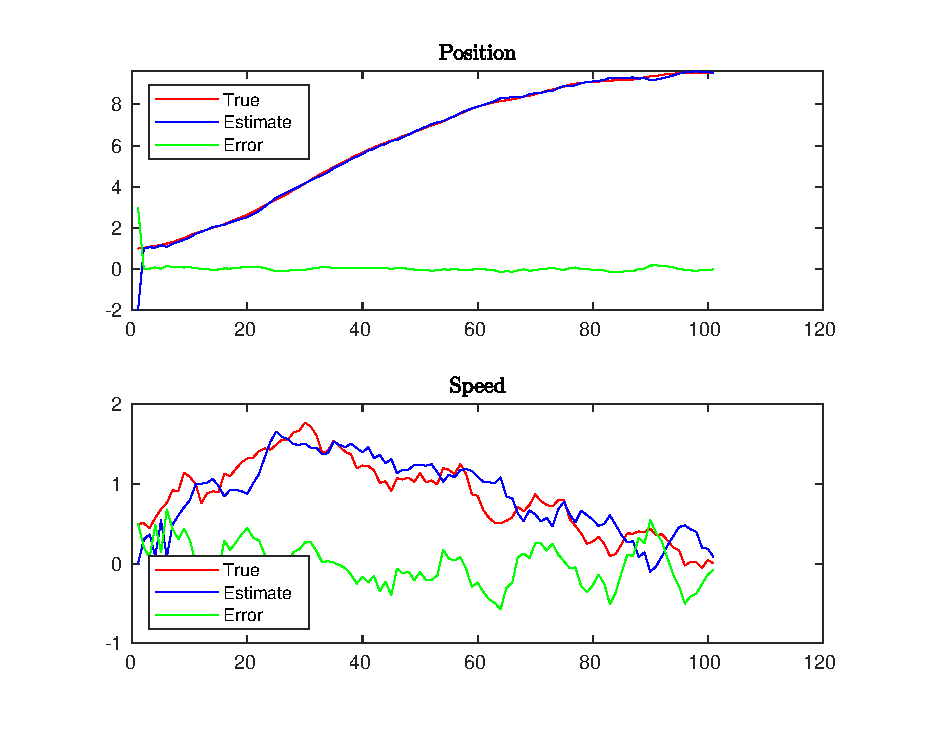
\includegraphics[width=0.57\columnwidth]{Warmup_Figure_1_wP_0_01_wV_0_1_vP_0_1.eps}
			\caption{Default parameters: $wStdP = 0.01$, $wStdV = 0.1$, and $vStd = 0.1$.}
			\label{fig:Warmup_Figure_1_wP_0_01_wV_0_1_vP_0_1}
		\end{figure}
			
		\begin{figure}[H]
			\centering
			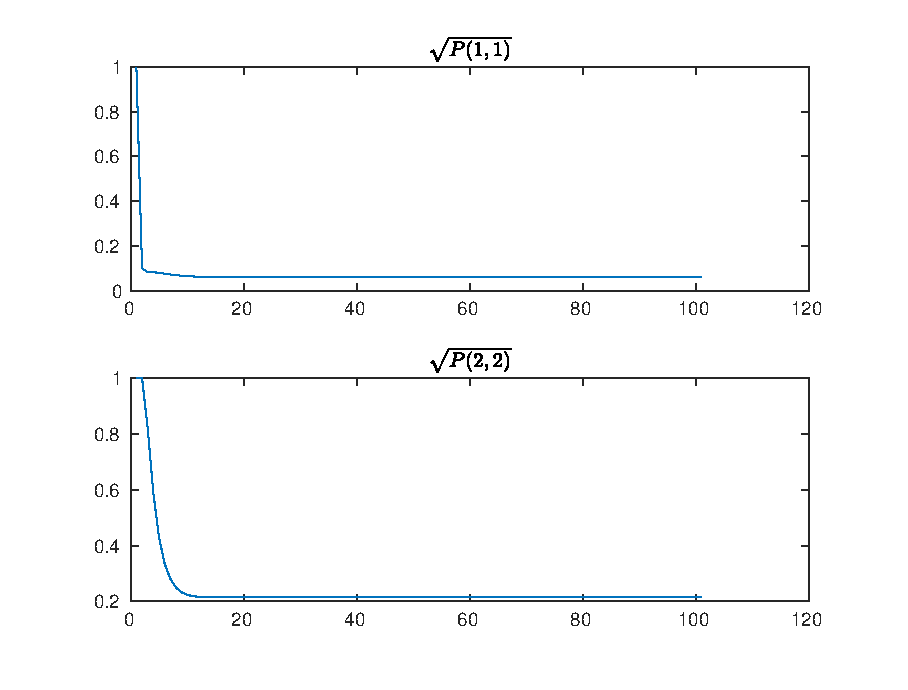
\includegraphics[width=0.57\columnwidth]{Warmup_Figure_2_wP_0_01_wV_0_1_vP_0_1.eps}
			\caption{Default parameters: $wStdP = 0.01$, $wStdV = 0.1$, and $vStd = 0.1$.}
			\label{fig:Warmup_Figure_2_wP_0_01_wV_0_1_vP_0_1}
		\end{figure}
		
		\begin{figure}[H]
			\centering
			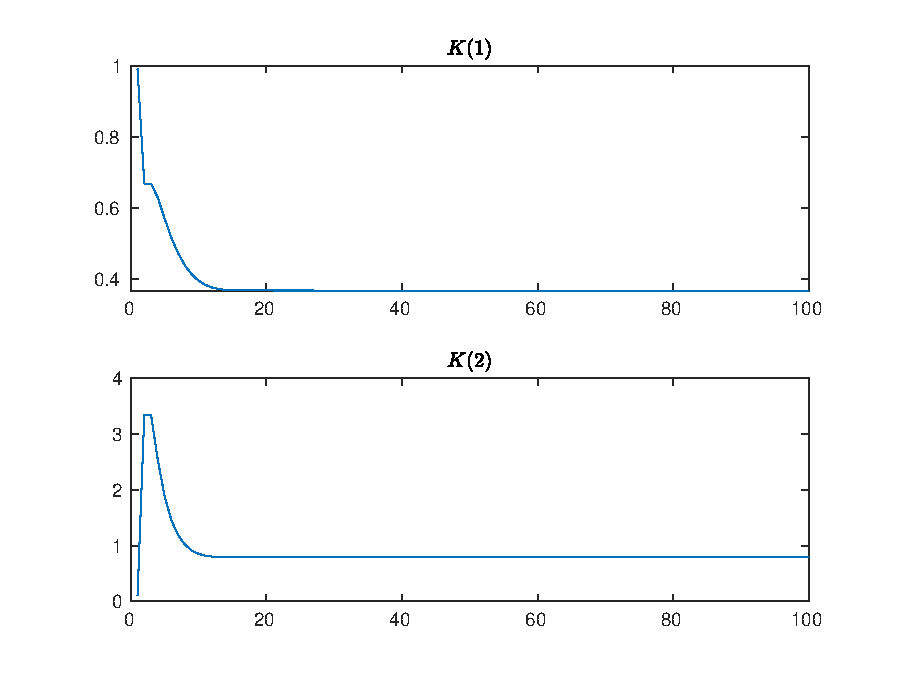
\includegraphics[width=0.57\columnwidth]{Warmup_Figure_3_wP_0_01_wV_0_1_vP_0_1.eps}
			\caption{Default parameters: $wStdP = 0.01$, $wStdV = 0.1$, and $vStd = 0.1$.}
			\label{fig:Warmup_Figure_3_wP_0_01_wV_0_1_vP_0_1}
		\end{figure}
		
		% Change measurement noise
		\begin{figure}[H]
			\centering
			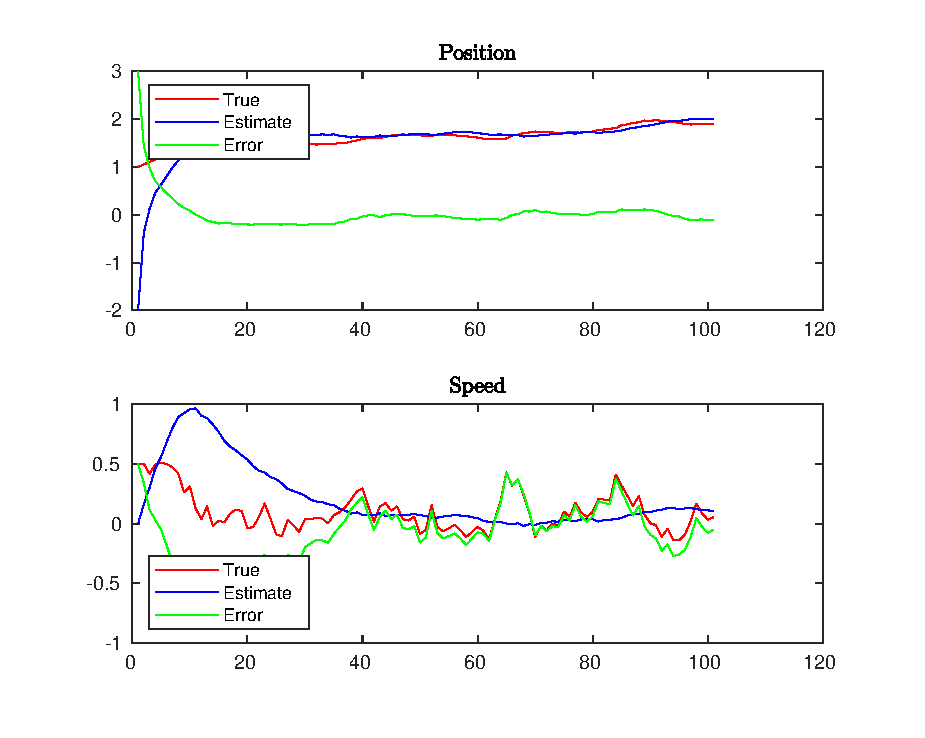
\includegraphics[width=0.57\columnwidth]{Warmup_Figure_1_wP_0_01_wV_0_1_vP_1.eps}
			\caption{Increase measurement noise: $wStdP = 0.01$, $wStdV = 0.1$, and $vStd = 1$.}
			\label{fig:Warmup_Figure_1_wP_0_01_wV_0_1_vP_1}
		\end{figure}
			
		\begin{figure}[H]
			\centering
			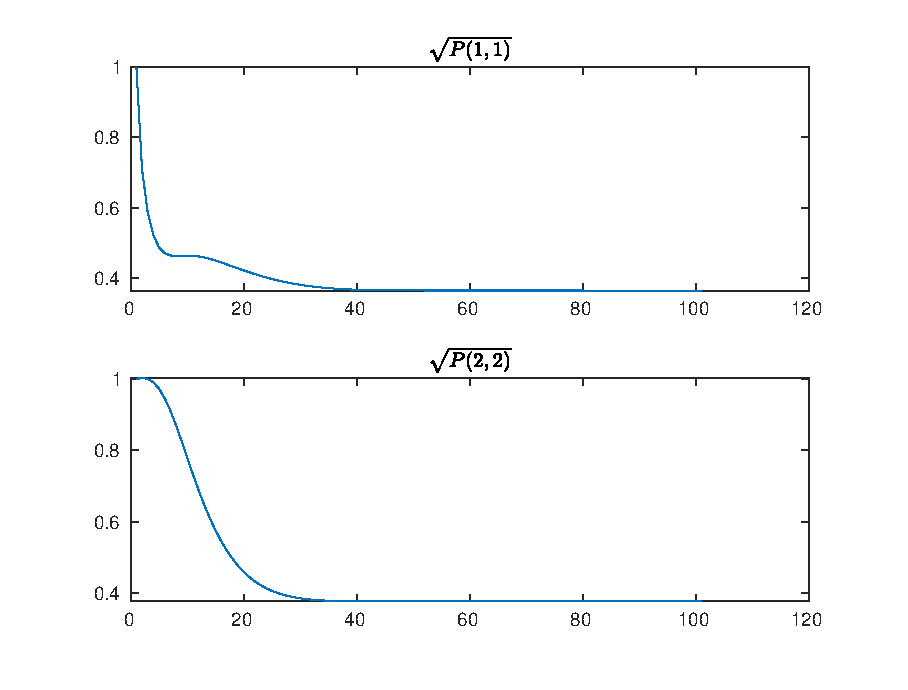
\includegraphics[width=0.57\columnwidth]{Warmup_Figure_2_wP_0_01_wV_0_1_vP_1.eps}
			\caption{Increase measurement noise: $wStdP = 0.01$, $wStdV = 0.1$, and $vStd = 1$.}
			\label{fig:Warmup_Figure_2_wP_0_01_wV_0_1_vP_1}
		\end{figure}
		
		\begin{figure}[H]
			\centering
			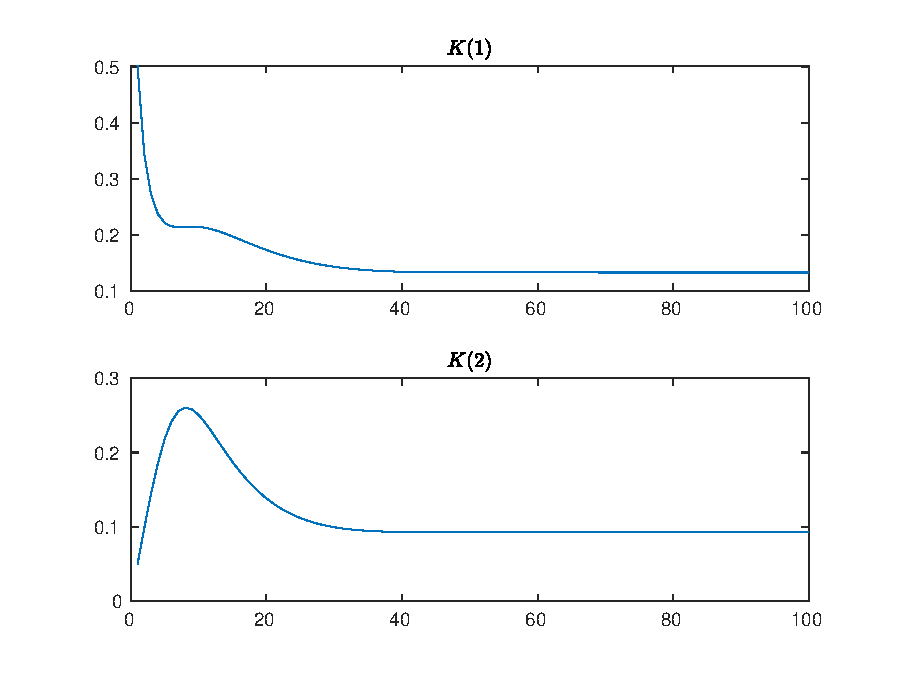
\includegraphics[width=0.57\columnwidth]{Warmup_Figure_3_wP_0_01_wV_0_1_vP_1.eps}
			\caption{Increase measurement noise: $wStdP = 0.01$, $wStdV = 0.1$, and $vStd = 1$.}
			\label{fig:Warmup_Figure_3_wP_0_01_wV_0_1_vP_1}
		\end{figure}
		
		% Change process noise
		\begin{figure}[H]
			\centering
			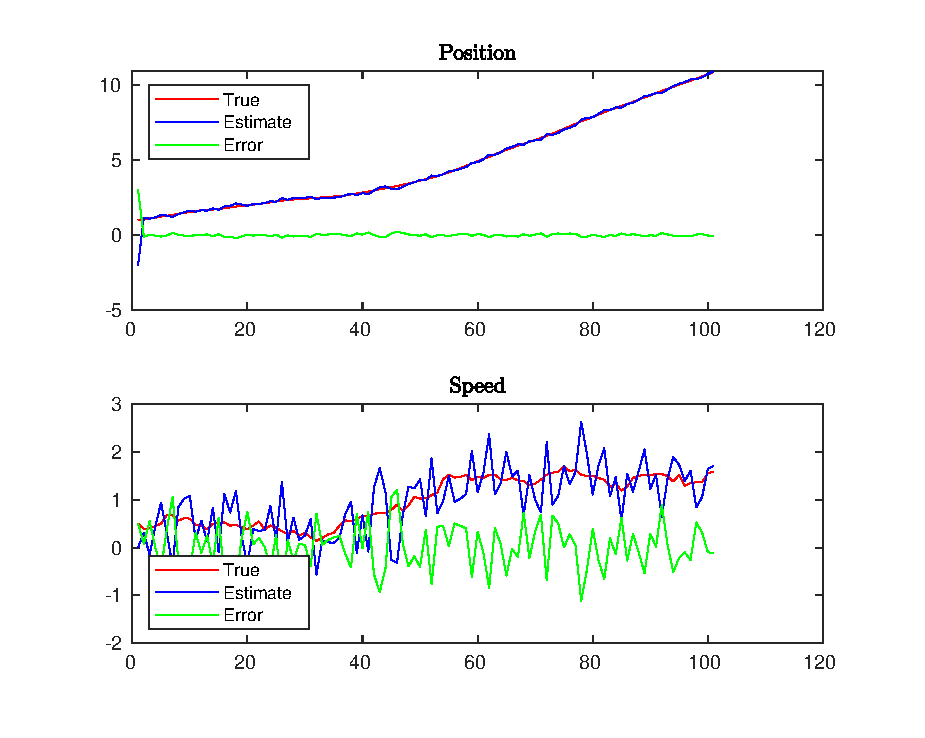
\includegraphics[width=0.57\columnwidth]{Warmup_Figure_1_wP_0_1_wV_1_vP_0_1.eps}
			\caption{Increase process noise: $wStdP = 0.1$, $wStdV = 1$, and $vStd = 0.1$.}
			\label{fig:Warmup_Figure_1_wP_0_1_wV_1_vP_0_1}
		\end{figure}
			
		\begin{figure}[H]
			\centering
			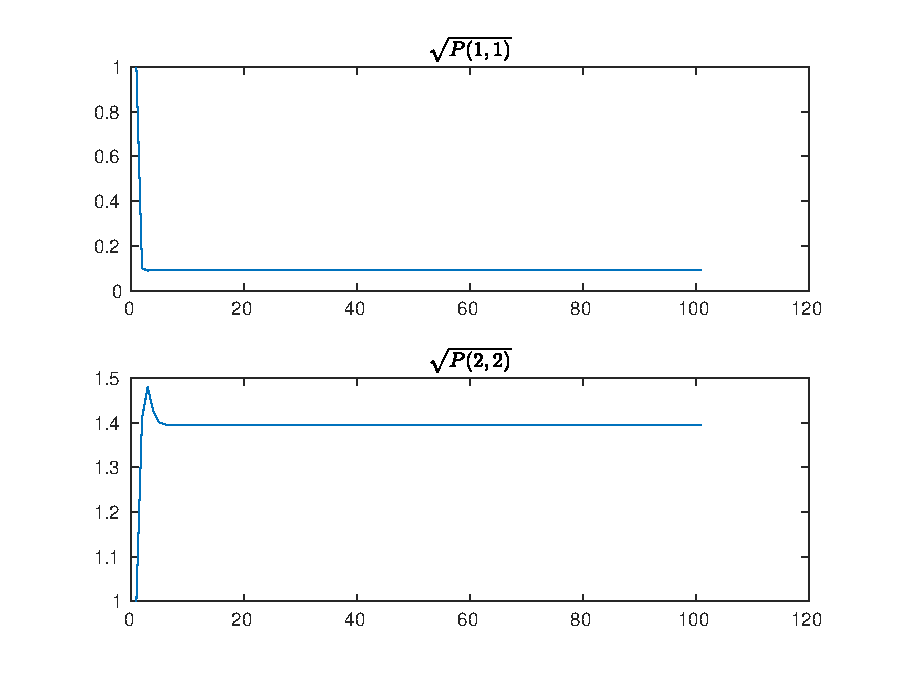
\includegraphics[width=0.57\columnwidth]{Warmup_Figure_2_wP_0_1_wV_1_vP_0_1.eps}
			\caption{Increase process noise: $wStdP = 0.1$, $wStdV = 1$, and $vStd = 0.1$.}
			\label{fig:Warmup_Figure_2_wP_0_1_wV_1_vP_0_1}
		\end{figure}
		
		\begin{figure}[H]
			\centering
			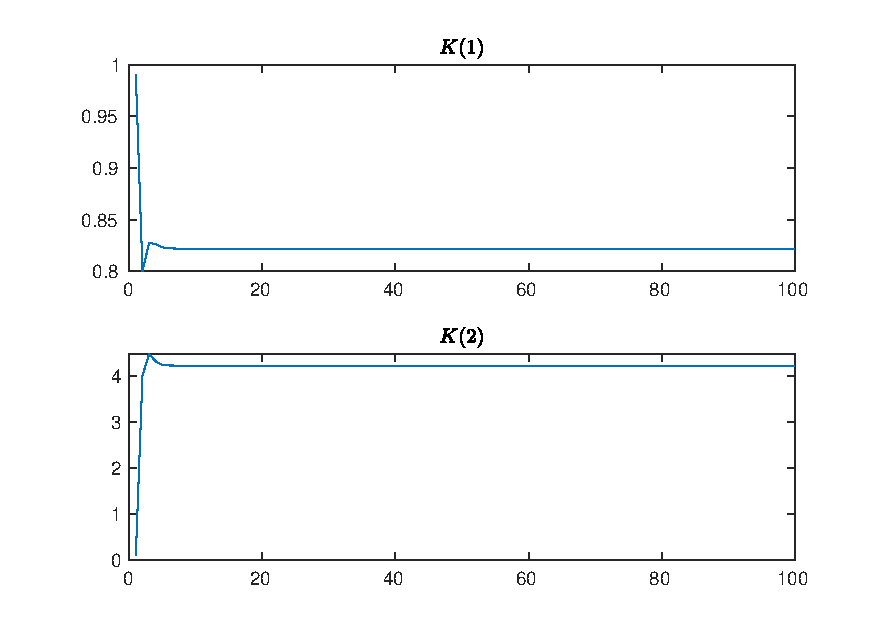
\includegraphics[width=0.57\columnwidth]{Warmup_Figure_3_wP_0_1_wV_1_vP_0_1.eps}
			\caption{Increase process noise: $wStdP = 0.1$, $wStdV = 1$, and $vStd = 0.1$.}
			\label{fig:Warmup_Figure_3_wP_0_1_wV_1_vP_0_1}
		\end{figure}
		
		% Change both noises
		\begin{figure}[H]
			\centering
			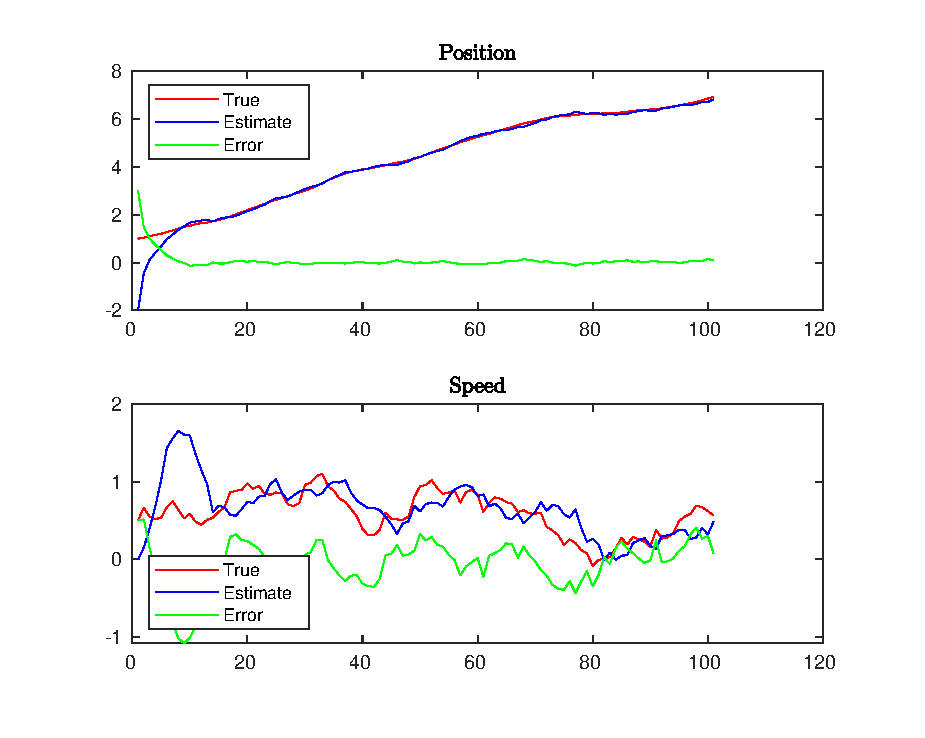
\includegraphics[width=0.57\columnwidth]{Warmup_Figure_1_wP_0_1_wV_1_vP_1.eps}
			\caption{Increase both noises: $wStdP = 0.1$, $wStdV = 1$, and $vStd = 1$.}
			\label{fig:Warmup_Figure_1_wP_0_1_wV_1_vP_1}
		\end{figure}
			
		\begin{figure}[H]
			\centering
			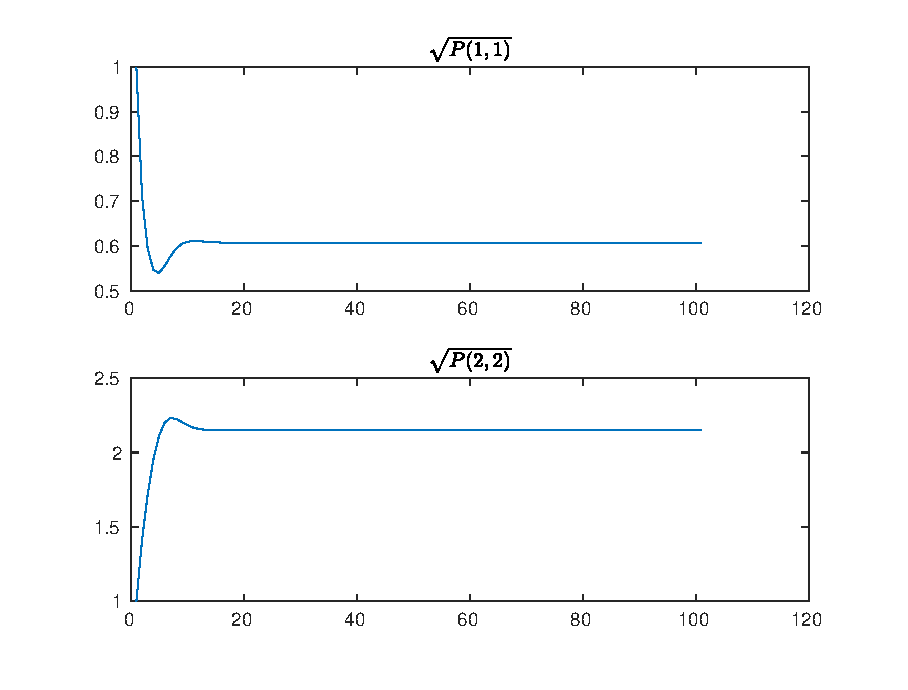
\includegraphics[width=0.57\columnwidth]{Warmup_Figure_2_wP_0_1_wV_1_vP_1.eps}
			\caption{Increase both noises: $wStdP = 0.1$, $wStdV = 1$, and $vStd = 1$.}
			\label{fig:Warmup_Figure_2_wP_0_1_wV_1_vP_1}
		\end{figure}
		
		\begin{figure}[H]
			\centering
			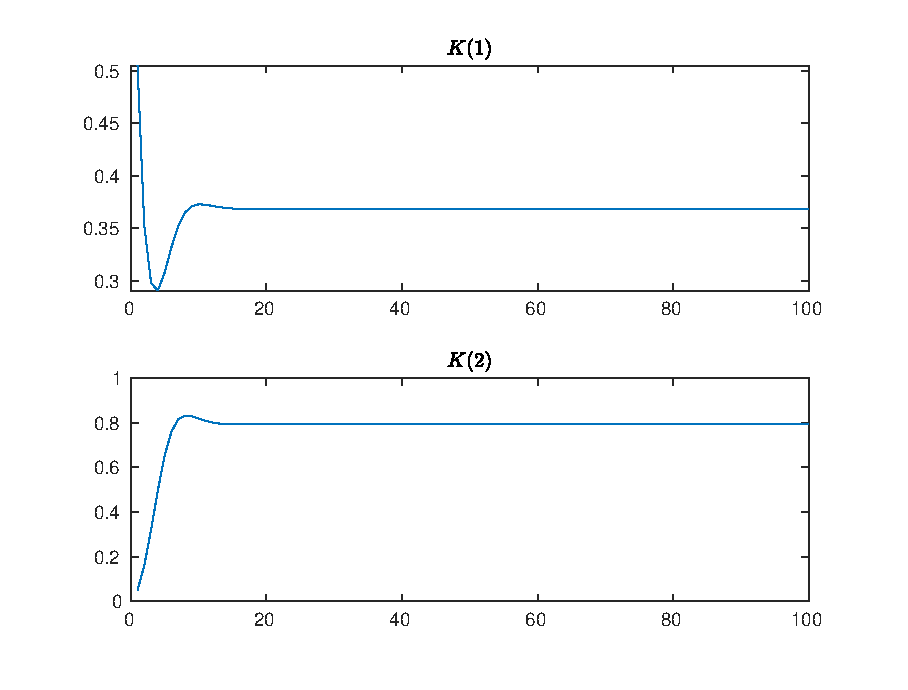
\includegraphics[width=0.57\columnwidth]{Warmup_Figure_3_wP_0_1_wV_1_vP_1.eps}
			\caption{Increase both noises: $wStdP = 0.1$, $wStdV = 1$, and $vStd = 1$.}
			\label{fig:Warmup_Figure_3_wP_0_1_wV_1_vP_1}
		\end{figure}

	% Question 4
	\item \addtocounter{cnt_questions}{1} \textbf{Question \arabic{cnt_questions}:} How do the initial values for $P$ and $xhat$ affect the rate of convergence and the error of the estimates (try both much bigger and much smaller)?
		\par If the initial value of $P$ is large, the uncertainty of the true state would be large and also the Kalman gain would be large. Meaning the measurement would have large weight. So the convergence time would not be affected largely. Also, the error of the estimates would not change much. The result is illustrated in Figure \ref{fig:Warmup_P_big}.
		\par If the initial value of $P$ is small, the system would have more confidence in the prediction, so the Kalman gain would increase slower, thus the convergence time would be longer. Also, the error of the estimates would not be changed much. The result is illustrated in Figure \ref{fig:Warmup_P_small}.
		\begin{figure}[H]
			\centering
			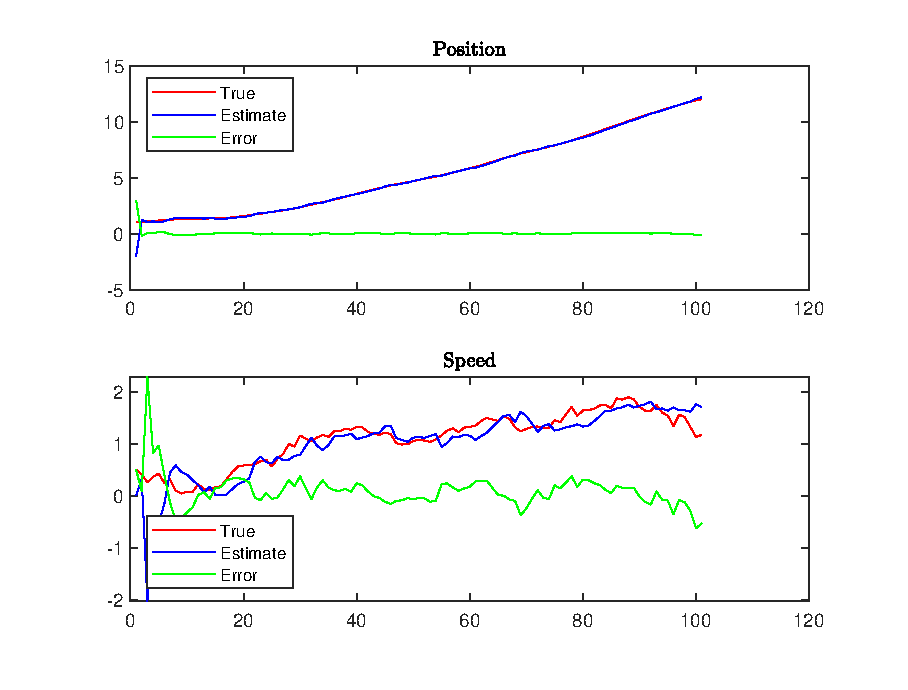
\includegraphics[width=0.71\columnwidth]{Figure/Warmup_P_big.eps}
			\caption{Increase $P$ to the 100 times of the original values.}
			\label{fig:Warmup_P_big}
		\end{figure}

		\begin{figure}[H]
			\centering
			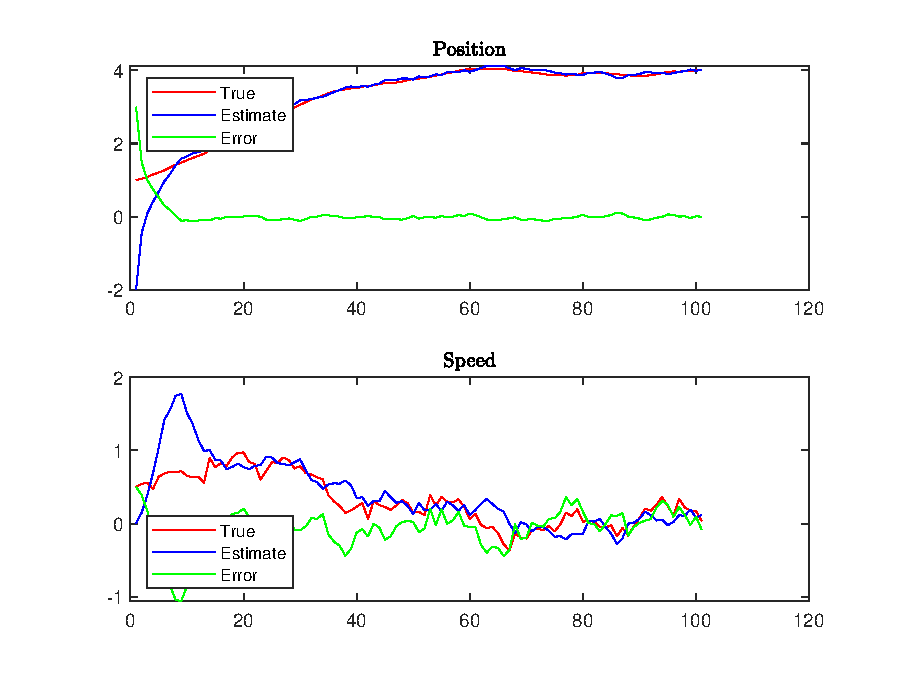
\includegraphics[width=0.71\columnwidth]{Figure/Warmup_P_small.eps}
			\caption{Decease $P$ to the 0.01 times of the original values.}
			\label{fig:Warmup_P_small}
		\end{figure}

		\par The initial values for $xhat$ would not affect the rate of convergence in a obvious way. Also, it would not obviously affect the error of the estimates. The results are illustrated in Figure \ref{fig:Warmup_xhat_big} and \ref{fig:Warmup_xhat_small}.
		\begin{figure}[H]
			\centering
			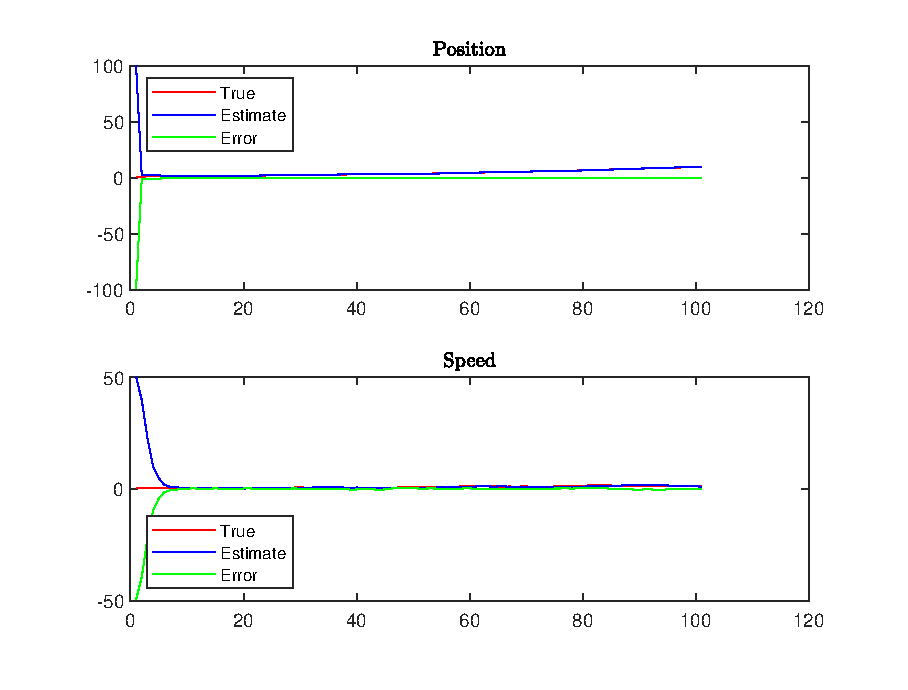
\includegraphics[width=0.86\columnwidth]{Warmup_xhat_big.eps}
			\caption{Increase $xhat$ to $[100;50]$.}
			\label{fig:Warmup_xhat_big}
		\end{figure}

		\begin{figure}[H]
			\centering
			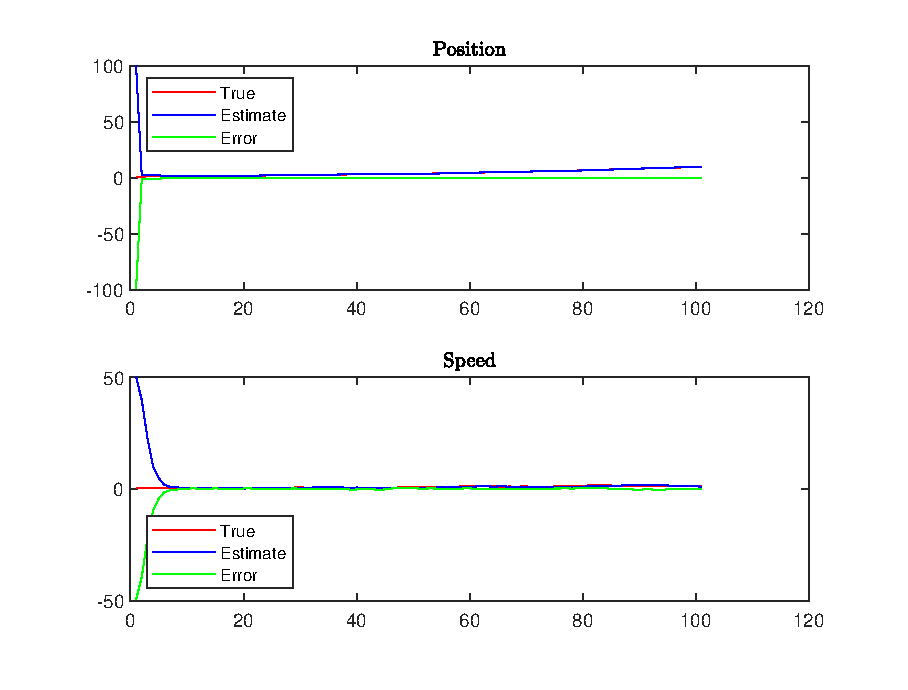
\includegraphics[width=0.86\columnwidth]{Warmup_xhat_big.eps}
			\caption{Decrease $xhat$ to $[1.5;0.75]$ which is close to the true position and velocity.}
			\label{fig:Warmup_xhat_small}
		\end{figure}
\end{itemize}

% -------------------------------------------------- %
\subsection{Main problem: EKF Localization}
\par Using a first order Markov assumption and Bayesian update:
\begin{equation}
\label{eq:rec_loc}
	\begin{split}
		\left\{
		\begin{array}{ll}
			p({\bf x_t} | {\bf u_{1:t}},{\bf z_{1:t}}, {\bf\bar x_0} ,M) & = \eta p({\bf z_t} | {\bf x_t},M)\int p({\bf x_t}|{\bf u_t},{\bf x_{t-1}}) p({\bf x_{t-1}}|{\bf z_{1:t-1}}, {\bf u_{1:t-1}}, {\bf\bar x_0},M)  {\bf dx_{t-1}}\\
			p(\bf x_0|\bar x_0 ) & = \delta(\bf x_0-\bar x_0)
		\end{array}
		\right.
	\end{split}
\end{equation} 
or equivalently
\begin{equation}
\label{eq:rec_loc_eq}
	\begin{split}
		\left\{
		\begin{array}{ll}
			bel(\bf x_t) &= p({\bf x_t|u_{1:t},z_{1:t},\bar x_0},M) = \eta p({\bf z_t|x_t},M)\overline{bel}(\bf x_t)\\
			\overline{bel}(\bf x_t) &= p({\bf x_t|u_{1:t},z_{1:t-1},\bar x_0},M) = \int p({\bf x_t|u_t,x_{t-1}}) bel({\bf x_{t-1}) dx_{t-1}}\\
			bel(\bf x_0) & = p({\bf x_0|\bar x_0} ) = \delta({\bf x_0-\bar x_0})
		\end{array}
		\right.
	\end{split}
\end{equation}
\begin{itemize}
	\item \addtocounter{cnt_questions}{1} \textbf{Question \arabic{cnt_questions}:} Which parts of (\ref{eq:rec_loc}) and (\ref{eq:rec_loc_eq}) are responsible for prediction and update steps?
		\par In Equation (\ref{eq:rec_loc_eq}) as the example, the first line of the equation is responsible for the update step. The second line of the equation is responsible for the prediction steps. While in Equation (\ref{eq:rec_loc}), the first line of the equation is responsible for both of the prediction and update steps.
\end{itemize}

\subsubsection{Maximum Likelihood Data Association}
\begin{itemize}
	\item \addtocounter{cnt_questions}{1} \textbf{Question \arabic{cnt_questions}:} In the maximum likelihood data association, we assumed that the measurements are independent of each other. Is this a valid assumption? Explain why.
		\par It is valid to assume that the measurements are independent of each other. The reason is that, the measurement model for each landmark at each time stamp only depends on the landmark, and the state at this time stamp, thus the measurement noise is white Gaussian noise and the covariance matrix of the measurement noise is diagonal meaning all the measurements are uncorrelated with each other.
\end{itemize}

\subsubsection{Outlier Detection}
\par It is possible to define a threshold on the Mahalanobis distance between the measurement($z^i_t$) and the most likely association which is given by:
\begin{equation}
	D_{M} = (\boldsymbol{\bar\nu}^i_t)^T(\bar S_{t,i})^{-1}(\boldsymbol{\bar\nu}^i_t)
	\label{eq:mahalanobis}
\end{equation}
\par $D_M$ follows the chi square ($X^{-2}_n$) cumulative distribution with n degree of freedom and therefore threshold be defined basing on a probability. $\nu$ has two degrees of freedom in our case, the threshold ($\lambda_M$) is given by:
\begin{equation}
	\lambda_M = X^{-2}_2(\delta_M)
	\label{eq:lambda}
\end{equation}

\begin{itemize}
	\item \addtocounter{cnt_questions}{1} \textbf{Question \arabic{cnt_questions}:} What are the bounds for $\delta_M$ in (\ref{eq:lambda})? How does the choice of $\delta_M$ affect the outlier rejection process? What value do you suggest for $\lambda_M$ when we have reliable measurements all arising from features in our map, that is all our measurements come from features on our map? What about a scenario with unreliable measurements with many arising from so called clutter or spurious measurements?
		\par The bounds for $\delta_M$ in (\ref{eq:lambda}) are $\delta_{M} \in [0, 1]$. Since the inverse chi square $\mathcal{X}^{-2}_{n}$ cumulative distribution is monotonically increasing, the increase in $\delta_{M}$ would result in the increase of the threshold $\lambda_{M}$. The larger the threshold $\lambda_{M}$, the more confidence would the system have on the measurement and the less measurements would be rejected as outliers. When we have reliable measurements come from features on our map, the covariance matrix for measurement noise would be small and few measurement should be viewed as outliers, so the threshold $\lambda_{M}$ should be large. On the contrast, when the measurements are unreliable, the threshold $\lambda_{M}$ should be small.
\end{itemize}

\subsubsection{Update}
\par The most simple type of update namely sequential update, performs one update for each observation $z^i_t$ in the $t^{th}$ time step (Algorithm \ref{alg:sequential_update}).

\begin{algorithm}
	\begin{algorithmic}
	\FORALL{Observations $i$ in $z_t$}
	\STATE $
	\begin{array}{lll}
		...&&\COMMENT{\texttt{Compute the $i^{th}$ association using $\boldsymbol{\bar\mu_t}$}}\\
		K_{t,i} &=& \bar \Sigma_t (\bar H_{t,i})^T (\bar S_{t,i})^{-1}\\
		\boldsymbol{\bar\mu}_{t} &=& \boldsymbol{\bar\mu}_{t} + K_{t,i} \boldsymbol{\bar\nu}^i_t\\
		\bar\Sigma_t &=& (I-K_{t,i} \bar H_{t,i})\bar\Sigma_t
	\end{array}
	$
	\ENDFOR
	\STATE
	$
	\begin{array}{lll}
	\boldsymbol\mu_t &=& \boldsymbol{\bar\mu}_{t}\\
	\Sigma_t &=& \bar\Sigma_t
	\end{array}
	$
	\end{algorithmic}
	\caption{Sequential update algorithm for the $i^{th}$ observation}
	\label{alg:sequential_update}
\end{algorithm}

\begin{itemize}
	\item \addtocounter{cnt_questions}{1} \textbf{Question \arabic{cnt_questions}:} Can you think of some down-sides of the sequential update approach (Algorithm \ref{alg:sequential_update})? Hint: How does the first noisy measurements affect the intermediate results?
		\par Since the first measurements are noisy and would result in non-zero innovations in the data association step. The non-zero (or not close to zero) innovation would cause the shift of the estimated mean. Also the noisy measurements would cause the covariance matrix $\bar{\Sigma}$ being reduced much more, thus resulting in smaller $S_{t,j}$ and higher Kalman gain in future time stamps. Then the Mahalanobis distance would increase and more reasonable measurements would be rejected as outliers.
\end{itemize}

\subsubsection{Batch Update}
An alternative to the sequential update is the batch update algorithm. Algorithm \ref{alg:batch_update} shows the complete EKF localization problem with the batch update.

\begin{itemize}
	\item \addtocounter{cnt_questions}{1} \textbf{Question \arabic{cnt_questions}:} How can you modify Algorithm \ref{alg:batch_update} to avoid redundant re-computations?
		\par In the Algorithm \ref{alg:batch_update}, ${\bf\hat z}_{t,j}$, $H_{t,j}$, and $S_{t,j}$ do not depend on the observation $z_{t}$ while still appear in the loop of $z_{t}$ which is causing redundant re-computations and can be avoided by taking them out of the $z_{t}$ loop so that these three parameters would be calculated only in the $M$ loop.
	
	\item \addtocounter{cnt_questions}{1} \textbf{Question \arabic{cnt_questions}:} What are the dimensions of $\boldsymbol{\bar\nu}_{t}$ and $\bar H_t$ in Algorithm \ref{alg:batch_update}? What were the corresponding dimensions in the sequential update algorithm? What does this tell you?
		\par The dimension of $\boldsymbol{\bar{\nu}^{i}}_{t}$ is of $2 \times 1$, so the dimension of $\boldsymbol{\bar{\nu}}_{t}$ is of $2n \times 1$, where $n$ is the number of inliers.
		\par The dimension of $\bar{H}_{t,i}$ is of $2 \times 3$, so the dimension of $\bar H_t$ is of $2n \times 3$, where $n$ is the number of inliers.
\end{itemize}

\begin{algorithm}[H]
	\begin{algorithmic}
	\FORALL{Observations $i$ in $z_t$}
	\FORALL{Landmarks $j$ in $M$}
	\STATE
	$
	\begin{array}{lll}
	{\bf\hat z}_{t,j} &=& {\bf h}(\boldsymbol{\bar\mu}_{t},M,j)\\
	H_{t,j} &=& H(\boldsymbol{\bar\mu}_{t}, M,j,{\bf\hat z}_{t,j})\\
	S_{t,j} &=& H_{t,j} \bar\Sigma_t (H_{t,j})^T + Q\\
	\boldsymbol{\nu}^{i,j}_{t} &=& \bf z_{t,i} - \hat z_{t,j}\\
	D^{i,j}_{t} &=& (\boldsymbol{\nu}^{i,j}_{t})^T(S_{t,j})^{-1}\boldsymbol\nu^{i,j}_{t}\\
	\psi^{i,j}_{t} & = & \det(2\pi S_{t,j})^{-\frac{1}{2}} exp[-\frac{1}{2}D^{i,j}_{t}]\\
	\end{array}
	$
	\ENDFOR
	\STATE
	$
	\begin{array}{lll}
	\hat c^i_t &=& \underset{j}{\arg\max \texttt{ }} \psi^{i,j}_{t}\\
	\hat o^i_t &=& D^{i,c^i_t} \geq \lambda_M \\
	\boldsymbol{\bar\nu}^i_t &=& \boldsymbol\nu^{i,\hat c^i_t}_{t}\\
	\bar H_{t,i} &=& H_{t,\hat c^i_t}
	\end{array}
	$
	\ENDFOR
	\STATE \COMMENT{For inlier indices $1,...,n$}
	\STATE
	$
	\begin{array}{lll}
	\boldsymbol{\bar\nu}_{t} &=& \left[
	\begin{array}{llll}
	(\boldsymbol{\bar\nu}^1_t)^T & (\boldsymbol{\bar\nu}^2_t)^T & ... & (\boldsymbol{\bar\nu}^n_t)^T
	\end{array}\right]^T \\
	\bar H_t &=&
	\left[
	\begin{array}{llll}
	(\bar H_{t,1})^T & (\bar H_{t,2})^T & ... & (\bar H_{t,n})^T
	\end{array}\right]^T \\
	\bar Q_t &=&
	\left[
	\begin{array}{llll}
		Q & 0& 0 & 0\\
		 0& Q & 0 & 0\\
		0& 0 & ... & 0\\
		0 & 0 & 0 & Q
	\end{array}
	\right]_{(2n \times 2n)} \\
	K_t &=& \bar \Sigma_t (\bar H_t)^T (\bar H_t \bar \Sigma_t (\bar H_t)^T + \bar Q_t)^{-1}\\
	{\boldsymbol\mu}_{t} &=& \boldsymbol{\bar\mu}_{t} + K_t\boldsymbol{\bar\nu}_{t}\\
	\Sigma_t &=& (I-K_t \bar H_t)\bar\Sigma_t
	\end{array}
	$
	\end{algorithmic}
	\caption{EKF Localization with Batch update for the $i^{th}$ time step}
	\label{alg:batch_update}
\end{algorithm}

\newpage
\subsection{Data sets}
\subsubsection{map\_o3.txt + so\_o3\_ie.txt}
\par In this case, the covariance matrix of the process and measurement noises are:
\begin{align*}
	R &= \begin{bmatrix} 0 .01^{2} & 0 & 0 \\ 0 & 0.01^{2} & 0 \\ 0 & 0 & (\frac{2\pi}{360})^{2} \end{bmatrix} \\
	Q &= \begin{bmatrix} 0.01^{2} & 0 \\ 0 & (\frac{2\pi}{360})^{2} \end{bmatrix}
\end{align*}
\vspace{2cm}
\begin{figure}[H]
	\centering
	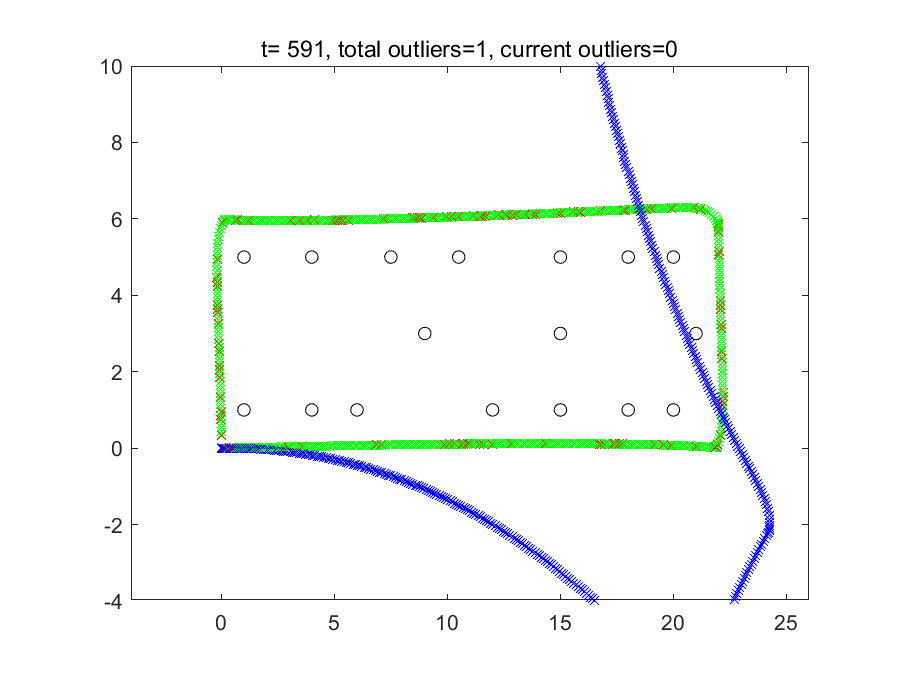
\includegraphics[width=\columnwidth]{Figure/Case_1_Figure_1.eps}
	\caption{Path in case 1.}
	\label{fig:Case_1_Figure_1}
\end{figure}

\begin{figure}[H]
	\centering
	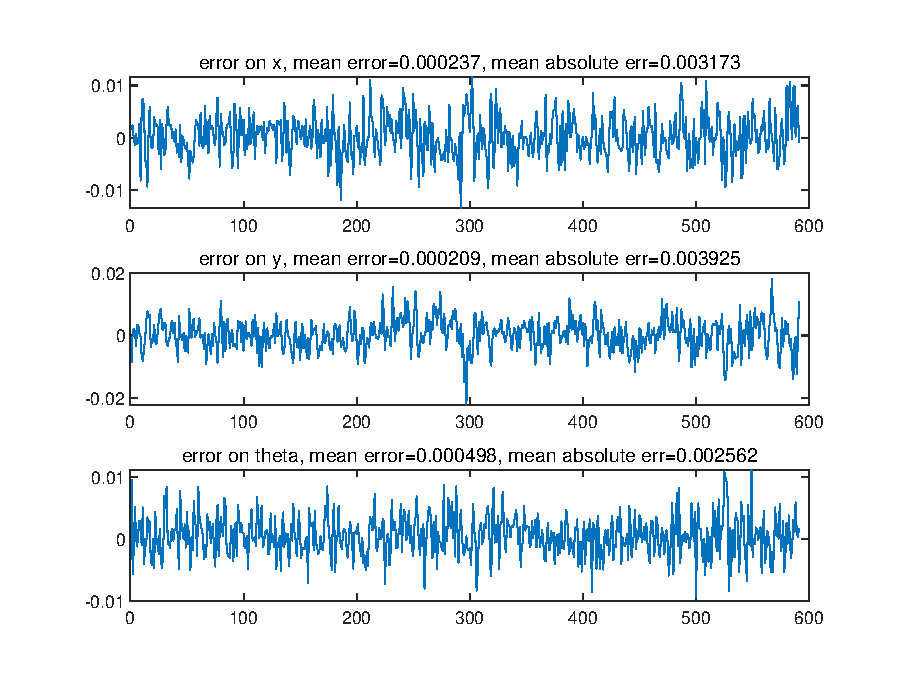
\includegraphics[width=0.9\columnwidth]{Figure/Case_1_Figure_2.eps}
	\caption{Error in case 1.}
	\label{fig:Case_1_Figure_2}
\end{figure}

\begin{figure}[H]
	\centering
	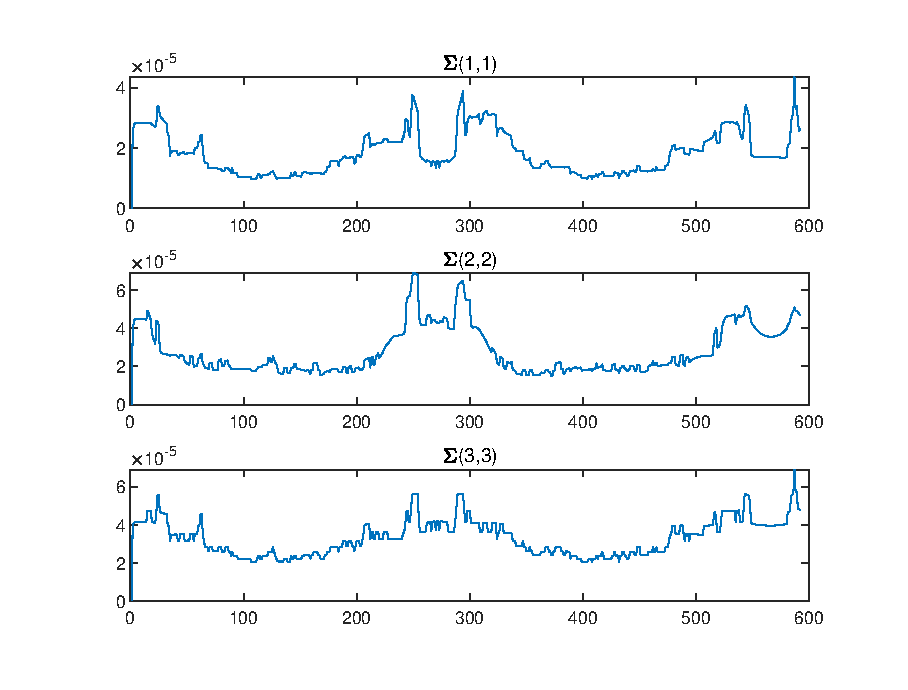
\includegraphics[width=0.9\columnwidth]{Figure/Case_1_Figure_3.eps}
	\caption{Covariance in case 1.}
	\label{fig:Case_1_Figure_3}
\end{figure}

\newpage
\subsubsection{map\_pent\_big\_10.txt + so\_pb\_10\_outlier.txt}
\par In this case, the covariance matrix of the process and measurement noises are:
\begin{align*}
	R &= \begin{bmatrix} 0 .01^{2} & 0 & 0 \\ 0 & 0.01^{2} & 0 \\ 0 & 0 & (\frac{2\pi}{360})^{2} \end{bmatrix} \\
	Q &= \begin{bmatrix} 0.2^{2} & 0 \\ 0 & 0.2^{2} \end{bmatrix}
\end{align*}
\vspace{2cm}
\begin{figure}[H]
	\centering
	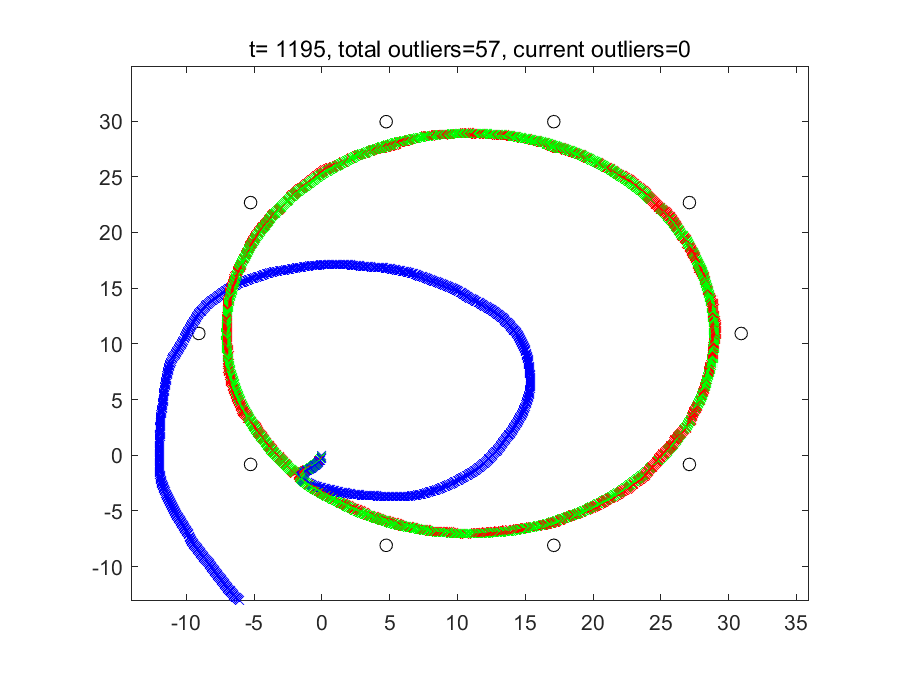
\includegraphics[width=\columnwidth]{Figure/Case_2_Figure_1.eps}
	\caption{Path in case 2.}
	\label{fig:Case_2_Figure_1}
\end{figure}

\begin{figure}[H]
	\centering
	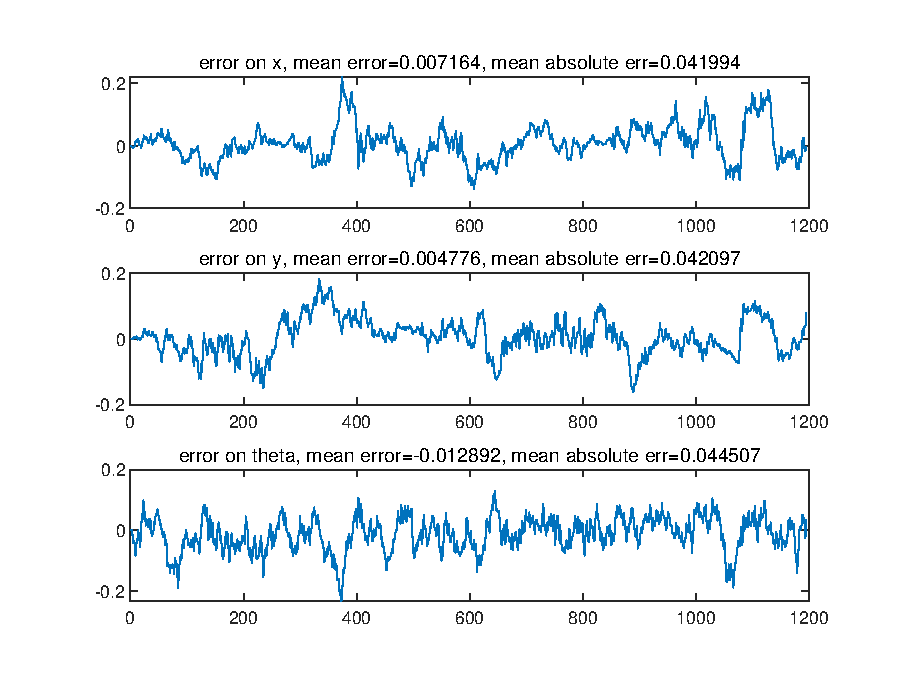
\includegraphics[width=0.9\columnwidth]{Figure/Case_2_Figure_2.eps}
	\caption{Error in case 2.}
	\label{fig:Case_2_Figure_2}
\end{figure}

\begin{figure}[H]
	\centering
	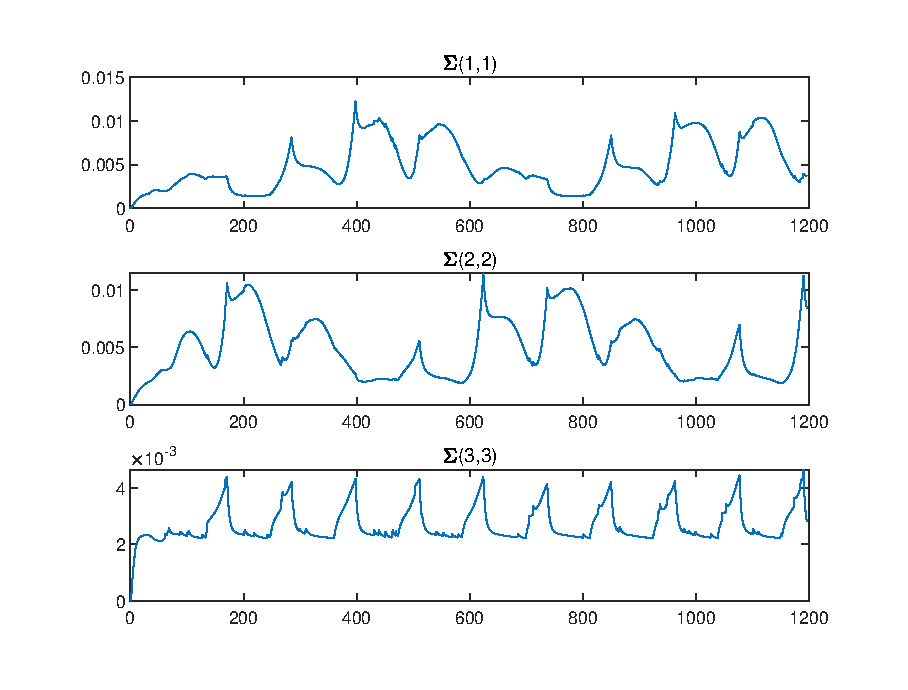
\includegraphics[width=0.9\columnwidth]{Figure/Case_2_Figure_3.eps}
	\caption{Covariance matrix in case 2.}
	\label{fig:Case_2_Figure_3}
\end{figure}

\newpage
\subsubsection{map\_pent\_big\_40.txt + so\_pb\_40\_no.txt}
\par In this case, the covariance matrix of the process and measurement noises are:
\begin{align*}
	R &= \begin{bmatrix} 1^{2} & 0 & 0 \\ 0 & 1^{2} & 0 \\ 0 & 0 & 1^{2} \end{bmatrix} \\
	Q &= \begin{bmatrix} 0.1^{2} & 0 \\ 0 & 0.1^{2} \end{bmatrix}
\end{align*}
also, the $\delta_{M}$ is set to 1.
\begin{itemize}
	\item Sequential update
		\vspace{2cm}
		\begin{figure}[H]
			\centering
			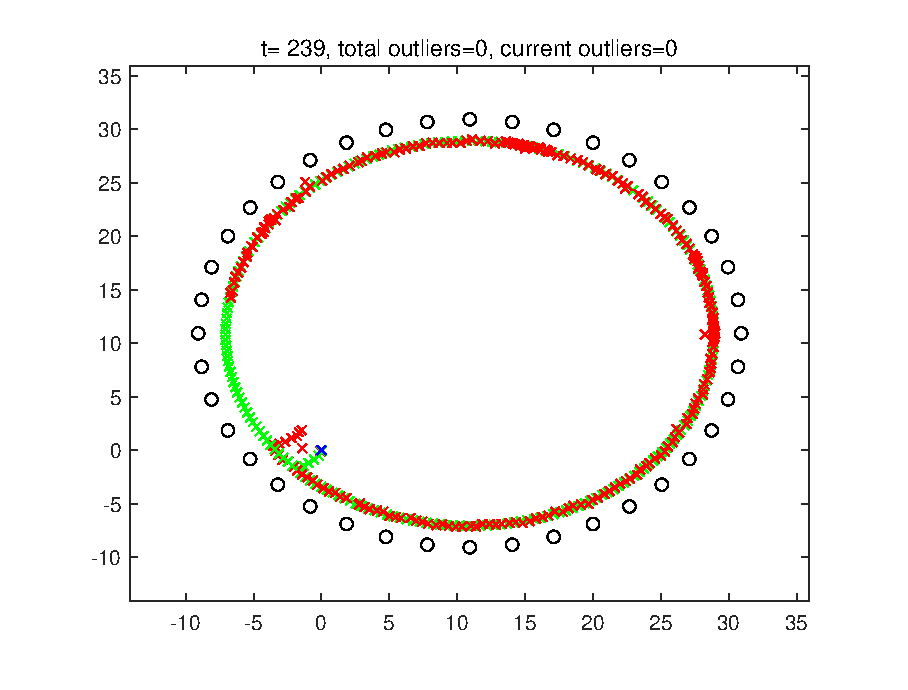
\includegraphics[width=\columnwidth]{Figure/Case_3_Figure_1.eps}
			\caption{Path in case 3.}
			\label{fig:Case_3_Figure_1}
		\end{figure}

		\begin{figure}[H]
			\centering
			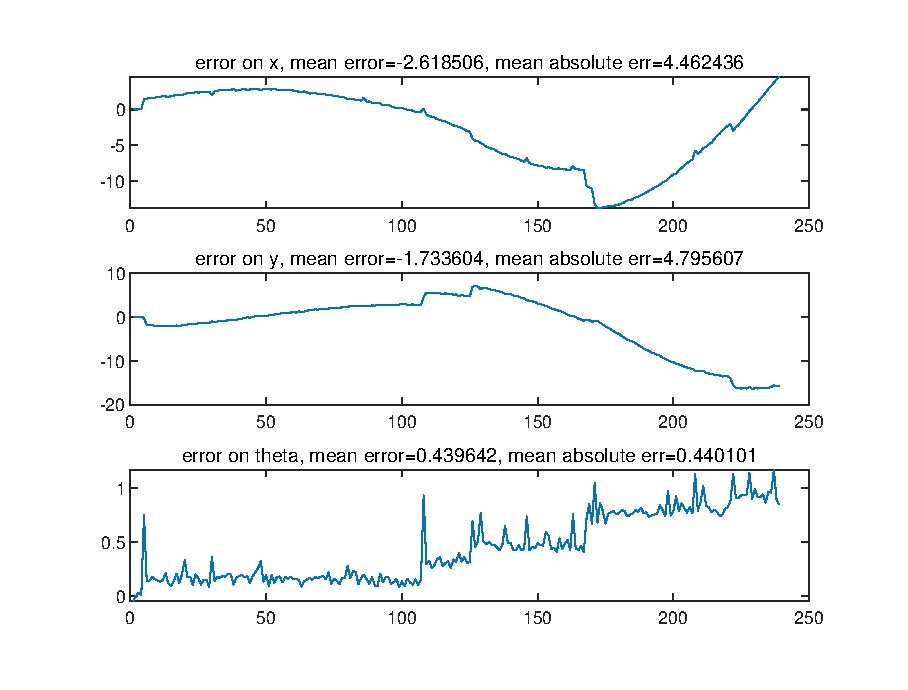
\includegraphics[width=0.9\columnwidth]{Figure/Case_3_Figure_2.eps}
			\caption{Error in case 3.}
			\label{fig:Case_3_Figure_2}
		\end{figure}

		\begin{figure}[H]
			\centering
			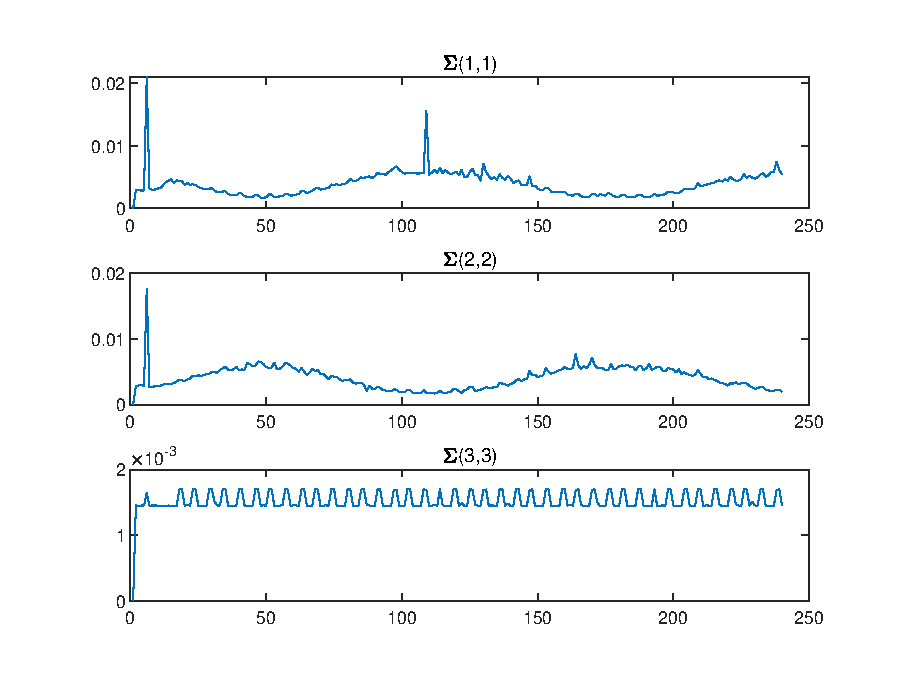
\includegraphics[width=0.9\columnwidth]{Figure/Case_3_Figure_3.eps}
			\caption{Covariance matrix in case 3.}
			\label{fig:Case_3_Figure_3}
		\end{figure}

	\item Batch update
		\begin{figure}[H]
			\centering
			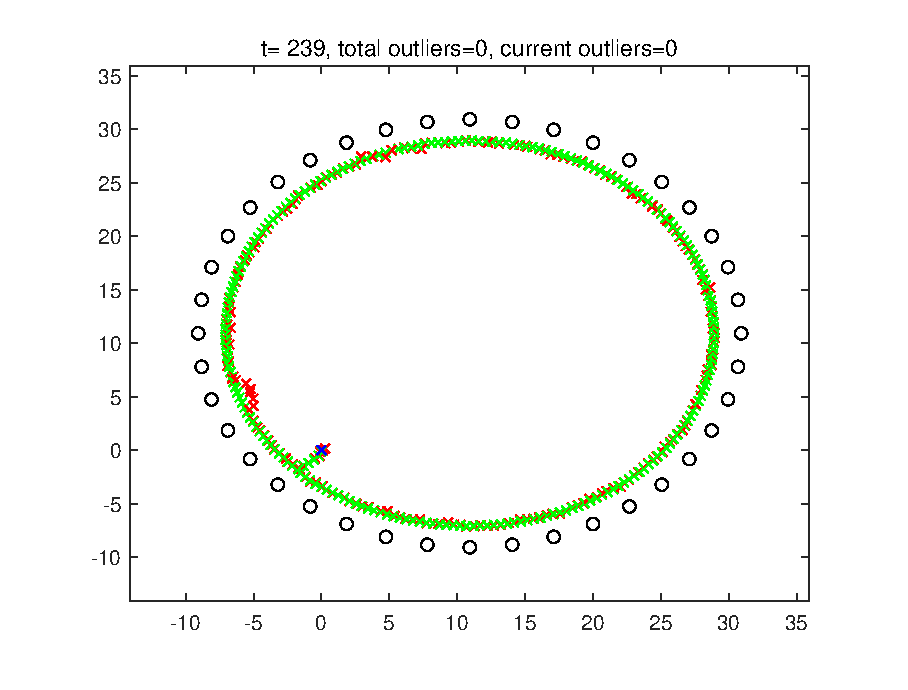
\includegraphics[width=0.9\columnwidth]{Figure/Case_3_Figure_1_Batch.eps}
			\caption{Path in case 3 with Batch update.}
			\label{fig:Case_3_Figure_1_Batch}
		\end{figure}

		\begin{figure}[H]
			\centering
			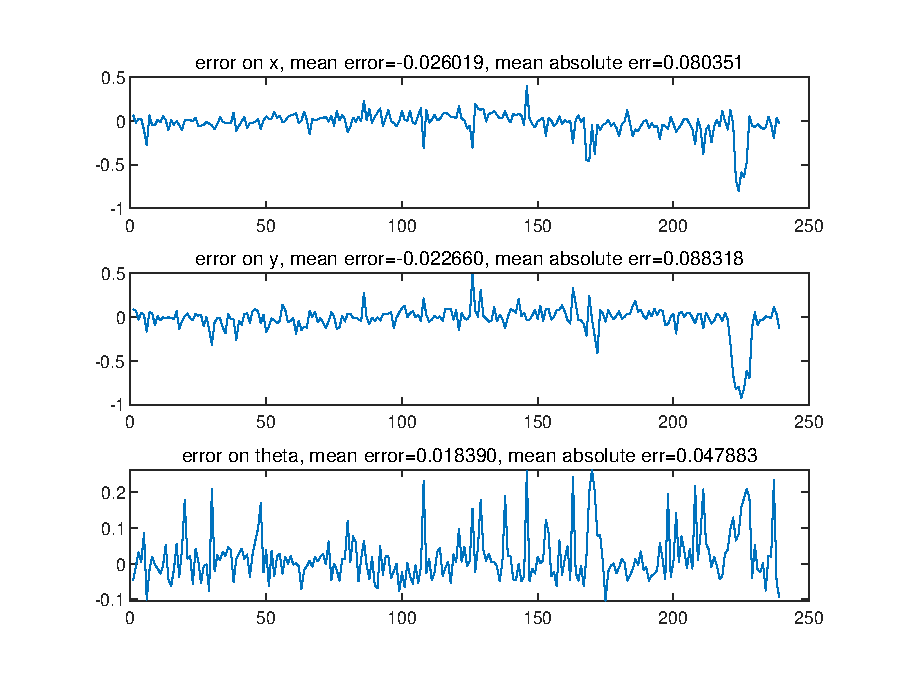
\includegraphics[width=0.9\columnwidth]{Figure/Case_3_Figure_2_Batch.eps}
			\caption{Error in case 3 with Batch update.}
			\label{fig:Case_3_Figure_2_Batch}
		\end{figure}

		\begin{figure}[H]
			\centering
			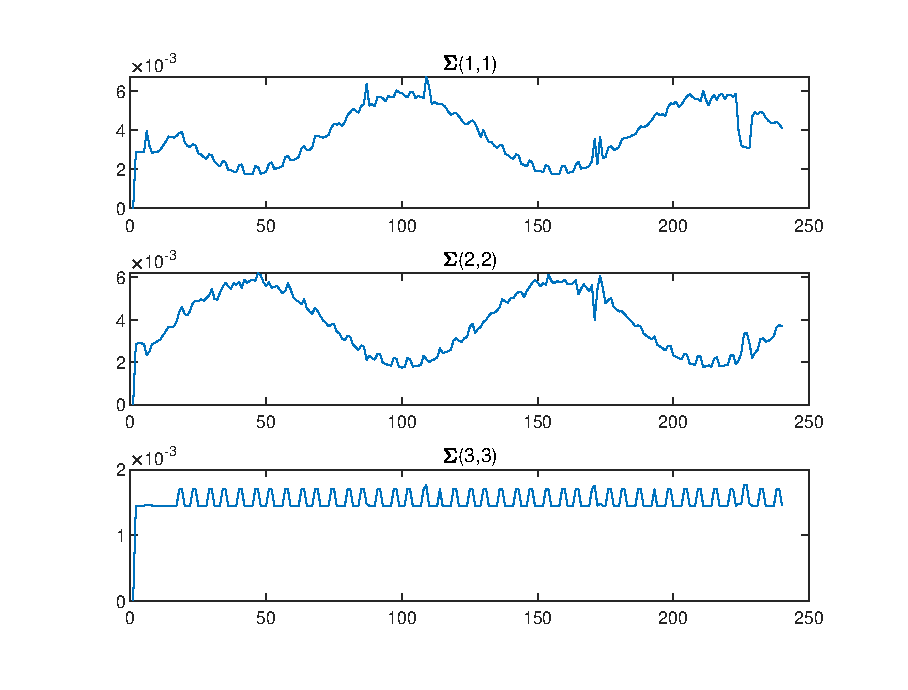
\includegraphics[width=\columnwidth]{Figure/Case_3_Figure_3_Batch.eps}
			\caption{Covariance matrix in case 3 with Batch update.}
			\label{fig:Case_3_Figure_3_Batch}
		\end{figure}
\end{itemize}

\end{document}